\documentclass[a4paper,12pt]{report}

% ============ PACCHETTI ============
\usepackage[utf8]{inputenc}
\usepackage[T1]{fontenc}
\usepackage[italian]{babel}
\usepackage{amsmath,amssymb,amsfonts}
\usepackage{graphicx}
\usepackage{booktabs}
\usepackage{hyperref}
\usepackage{geometry}
\usepackage{caption}
\usepackage{subcaption}
\usepackage{float}
\usepackage{enumitem}
\usepackage{xcolor}
\usepackage{listings}
\usepackage[section]{placeins}

% Ottimizzazione dei parametri di posizionamento dei float
\renewcommand{\topfraction}{0.85}
\renewcommand{\bottomfraction}{0.85}
\renewcommand{\textfraction}{0.15}
\renewcommand{\floatpagefraction}{0.8}
\setlist{itemsep=2pt, topsep=3pt, parsep=0pt}

\geometry{margin=2.5cm}

\hypersetup{
    colorlinks=true,
    linkcolor=blue!70!black,
    citecolor=green!50!black,
    urlcolor=blue!60!black
}

% Percorso delle immagini
\graphicspath{{Scripts/Task2_Object_Recognition/runs/detect/}}

\title{Progetto EGO-CH --- Deep Learning\\
\large Relazione Finale}
\author{Nome Cognome \and Nome Cognome \and Nome Cognome}
\date{Anno Accademico 2025/2026}

\begin{document}

\maketitle
\tableofcontents
\newpage

% ================================================================
% CAPITOLO 1 — INTRODUZIONE
% ================================================================
\chapter{Introduzione}

\section{Contesto e Motivazione}

Negli ultimi anni, la convergenza tra le tecnologie indossabili (\emph{wearable devices}) e l'Intelligenza Artificiale ha aperto nuove prospettive nel campo della fruizione del patrimonio culturale (\emph{Augmented Cultural Heritage}). La \textbf{Egocentric Vision} (o \emph{First-Person Vision}, FPV) si differenzia radicalmente dalla visione artificiale classica a telecamera fissa: catturando il mondo dalla prospettiva diretta dell'utente (<<what the user sees is what the camera captures>>), offre una finestra privilegiata sulle dinamiche di esplorazione, l'attenzione visiva e il comportamento spontaneo dei visitatori all'interno di musei e siti archeologici.

Il presente progetto accademico si colloca nell'ambito dei progetti nazionali e regionali \textbf{VEDI} (\emph{Vision Exploitation for Data Interpretation}) e \textbf{VALUE} (\emph{Visual Analysis for Localization and Understanding of Environments}), sviluppati dall'Image Processing Laboratory (IPLab) dell'Università di Catania in collaborazione con il centro di ricerca CUTGANA e partner industriali. L'obiettivo primario di tali iniziative è la creazione di sistemi di assistenza intelligente per visitatori (es. guide virtuali contestuali ed egocentriche) e di strumenti avanzati di business intelligence per i curatori museali, capaci di analizzare in tempo reale i percorsi di visita, i tempi di permanenza di fronte alle opere e il gradimento complessivo dell'esperienza culturale.

\section{La Visione Egocentrica nei Beni Culturali: Sfide Tecniche}

L'elaborazione automatica di video egocentrici acquisiti in contesti museali <<in-the-wild>> presenta una serie di sfide metodologiche estremamente complesse, che rendono inadeguati gli approcci convenzionali di Computer Vision:

\begin{itemize}
    \item \textbf{Ego-Motion e Motion Blur}: i movimenti naturali, rapidi e incontrollati del capo del visitatore introducono continue variazioni del punto di vista, inclinazioni della linea d'orizzonte e vistose sfocature da movimento (\emph{motion blur}).
    \item \textbf{Condizioni Illuminotecniche Cangianti}: le visite reali si svolgono nell'arco di intere giornate e stagioni differenti, esponendo le telecamere a sbalzi continui tra luce solare diretta (es. cortili o finestre), penombra di sale espositive e riflessi artificiali sui vetri di protezione delle opere.
    \item \textbf{Occlusioni Parziali e Prospettive Sghembe}: le opere d'arte vengono frequentemente inquadrate da angolazioni fortemente prospettiche, a distanze ravvicinate o parzialmente coperte dal passaggio di altri visitatori.
    \item \textbf{Riconoscimento a livello di Istanza (\emph{Instance-Level Recognition})}: a differenza dei benchmark di object detection tradizionali (es. COCO, Pascal VOC) incentrati sulla categorizzazione di classi generiche (es. ``persona'', ``sedia''), nei beni culturali il sistema deve discriminare tra \emph{singole istanze} visivamente affini (es. dipinti sacri dello stesso artista, affreschi del medesimo periodo storico o dettagli decorativi analoghi).
\end{itemize}

\section{Obiettivi della Ricerca e Struttura della Relazione}

Per stimolare la ricerca e fornire un benchmark di riferimento per la comunità scientifica, Ragusa et al.~\cite{egoref} hanno introdotto il dataset \textbf{EGO-CH}, definendo quattro task fondamentali per la comprensione del comportamento del visitatore:

\begin{enumerate}
    \item \textbf{Task 1 --- Room-based Localization}: la localizzazione frame-per-frame e la tracciatura sequenziale dell'ambiente (stanza) in cui si trova il visitatore all'interno del sito culturale.
    \item \textbf{Task 2 --- Point of Interest (POI) Recognition}: il rilevamento spaziale (\emph{object detection} tramite bounding box 2D) e la classificazione dei Punti di Interesse visibili nel campo visivo.
    \item \textbf{Task 3 --- Object Retrieval}: il recupero dell'immagine di riferimento pulita di un'opera d'arte a partire da una patch ritagliata da una query egocentrica (\emph{One-Shot Retrieval}).
    \item \textbf{Task 4 --- Survey Prediction}: la predizione automatica del questionario di gradimento e memoria compilato dal visitatore al termine della visita, basata sull'analisi del video egocentrico.
\end{enumerate}

L'obiettivo fondamentale della presente relazione è quello di superare i limiti delle baseline storiche proposte nel paper originale del 2020 (basate su architetture ormai datate quali VGG19, K-NN e YOLOv3), introducendo una pipeline di \textbf{Deep Learning di ultima generazione}. 

In particolare, abbiamo sfruttato l'espressività dei \textbf{Foundation Model basati su Vision Transformer} (\textbf{DINOv2}), l'efficienza dei modelli di sequenza a spazio di stato (\textbf{Mamba SSM}) e la precisione dei moderni detector anchor-free (\textbf{YOLOv8}), stabilendo il nuovo stato dell'arte su tutti e tre i task fondamentali del benchmark EGO-CH senza modificare il protocollo di valutazione originale.

La relazione è strutturata come segue:
\begin{itemize}
    \item Il \textbf{Capitolo 2} descrive in dettaglio l'architettura del dataset \textbf{EGO-CH}, i protocolli di acquisizione hardware, i due siti culturali considerati e la struttura delle annotazioni.
    \item Il \textbf{Capitolo 3} affronta il \textbf{Task 1 (Room-based Localization)}, presentando la pipeline basata su feature DINOv2 e sequence modeling temporale con Mamba.
    \item Il \textbf{Capitolo 4} analizza il \textbf{Task 2 (Point of Interest Recognition)}, illustrando l'approccio end-to-end con YOLOv8 nelle varianti Nano e X-Large.
    \item Il \textbf{Capitolo 5} presenta il \textbf{Task 3 (Object Retrieval)}, descrivendo il matching nello spazio latente di DINOv2 mediante Cosine Similarity e la risoluzione del \emph{Domain Shift}.
    \item Il \textbf{Capitolo 6} trae le \textbf{Conclusioni} finali e sintetizza i contributi complessivi del lavoro.
\end{itemize}


% ================================================================
% CAPITOLO 2 — IL DATASET EGO-CH
% ================================================================
\chapter{Il Dataset EGO-CH}

\section{Protocollo di Acquisizione e Hardware}

Il dataset \textbf{EGO-CH} (\emph{Egocentric Cultural Heritage})~\cite{egoref} è un benchmark di riferimento per la visione egocentrica nei beni culturali, progettato e raccolto dal gruppo di ricerca IPLab dell'Università di Catania.

Le acquisizioni sono state condotte impiegando visori indossabili \textbf{Microsoft HoloLens} di prima generazione, montati sulla testa dei partecipanti. Questo dispositivo permette di registrare il flusso video egocentrico garantendo che il centro della fotocamera sia costantemente allineato con la direzione prevalente dello sguardo dell'utente.

La campagna di acquisizione ha coinvolto un totale di \textbf{70 soggetti distinti}, suddivisi tra volontari (per le sessioni di addestramento) e \textbf{60 visitatori reali} non guidati (per le sessioni di test e valutazione comportamentale). Le riprese sono state distribuite nell'arco di \textbf{oltre tre mesi}, consentendo di catturare una naturale ed estesa variabilità delle condizioni ambientali (affollamento, illuminazione diurna e artificiale, percorsi di esplorazione non vincolati). Complessivamente, il dataset raccoglie \textbf{oltre 27 ore di video egocentrici ad alta risoluzione}.

\section{I Siti Culturali e Statistiche Dettagliate}

Le acquisizioni si sono svolte all'interno di due importanti ed eterogenei siti culturali situati in Sicilia:

\subsection{Palazzo Bellomo (Siracusa)}
La Galleria Regionale di Palazzo Bellomo a Siracusa ospita una vasta collezione d'arte medievale e moderna, disposta in una struttura architettonica complessa e articolata.
\begin{itemize}
    \item \textbf{Ambienti (Stanze)}: 22 sale espositive distinte.
    \item \textbf{Points of Interest (POI)}: 191 oggetti di interesse annotati (principalmente dipinti, sculture, iscrizioni e manufatti d'arte).
    \item \textbf{Video di Training}: 57 clip video di breve durata (media di 1.4 minuti per clip), incentrate su specifici POI o ambienti.
    \item \textbf{Video di Test}: 10 sequenze video continue a risoluzione $1280 \times 720$ pixel @ 29.97 fps, con una durata media di 31.3 minuti ciascuna, corrispondenti a visite integrali.
    \item \textbf{Annotazioni Spaziali}: 70.088 frame annotati manualmente con bounding box 2D.
    \item \textbf{Query Patch}: 23.727 immagini ritagliate dalle bounding box dei POI nei video di test.
    \item \textbf{Gallery di Riferimento}: 191 fotografie ufficiali da catalogo dei POI (1 immagine di alta qualità per ciascun POI).
\end{itemize}

\subsection{Monastero dei Benedettini (Catania)}
Il Monastero di San Nicolò l'Arena a Catania è un complesso monumentale tardo-barocco (patrimonio UNESCO) caratterizzato da ampi spazi architettonici.
\begin{itemize}
    \item \textbf{Ambienti (Stanze)}: 4 macro-ambienti espositivi e di transito (Antirefettorio, Refettorio Grande, Corridoio dell'Orologio, Chiostro).
    \item \textbf{Points of Interest (POI)}: 35 POI annotati. A differenza di Palazzo Bellomo, qui i POI comprendono sia opere d'arte che complessi \textbf{elementi architettonici} (es. portali monumentali, archi, pavimenti maiolicati, corridoi e scaloni).
    \item \textbf{Video di Training e Validation}: 48 video di training e 5 video di validation a risoluzione $1216 \times 684$ pixel @ 24 fps.
    \item \textbf{Visite Reali di Test}: 60 video di visite integrali condotte da 60 visitatori reali a risoluzione $1408 \times 792$ pixel @ 30.03 fps.
    \item \textbf{Annotazioni Spaziali}: 106.911 frame annotati con bounding box 2D.
    \item \textbf{Query Patch}: 44.978 immagini ritagliate dalle bounding box nei video di test.
    \item \textbf{Gallery di Riferimento}: 35 immagini di riferimento ufficiali dei POI.
    \item \textbf{Sondaggi (Surveys)}: 60 questionari completi di gradimento e memoria dei POI compilati dai visitatori al termine della visita.
\end{itemize}

La Tabella~\ref{tab:egoch_summary} sintetizza la struttura quantitativa dei due siti culturali appartenenti al benchmark.

\begin{table}[htbp]
\centering
\caption{Statistiche riassuntive del dataset EGO-CH per i due siti culturali.}
\label{tab:egoch_summary}
\resizebox{\textwidth}{!}{%
\begin{tabular}{lcc}
\toprule
\textbf{Proprietà} & \textbf{Palazzo Bellomo (Siracusa)} & \textbf{Monastero dei Benedettini (Catania)} \\
\midrule
Ambienti (Stanze)           & 22                  & 4 (5 etichette test) \\
Points of Interest (POI)    & 191                 & 35 \\
Soggetti coinvolti          & Volontari + Test    & 60 visitatori reali \\
Risoluzione Video           & $1280 \times 720$   & $1216 \times 684$ / $1408 \times 792$ \\
Frame annotati (BB)         & 70.088              & 106.911 \\
Patch visive estratte (Query)& 23.727             & 44.978 \\
Immagini Gallery (One-Shot) & 191                 & 35 \\
Sondaggi associati          & ---                 & 60 questionari reali \\
\bottomrule
\end{tabular}%
}
\end{table}

\section{Struttura delle Annotazioni}

Il dataset EGO-CH fornisce annotazioni ricche e multi-livello per supportare i diversi task di machine learning:

\begin{enumerate}
    \item \textbf{Annotazioni Temporali (\emph{Room e POI level})}: per ogni fotogramma $t$ dei video di visita, un file di annotazione specifica in quale stanza si trova il visitatore e se sta osservando direttamente uno dei POI codificati.
    \item \textbf{Annotazioni Spaziali (Bounding Boxes 2D)}: per i fotogrammi in cui sono visibili POI, sono fornite le coordinate rettangolari $(x_{\min}, y_{\min}, x_{\max}, y_{\max})$ che delimitano la posizione dell'oggetto nel frame.
    \item \textbf{Annotazioni di Sondaggio (\emph{Surveys})}: per le 60 visite del Monastero, ciascun visitatore ha indicato in un questionario finale se ricordava di aver visto ciascuno dei 35 POI e ha assegnato un punteggio di gradimento su una scala discreta da $-7$ a $+7$.
\end{enumerate}

\section{Analisi della Complessità e delle Criticità del Dominio}

L'analisi dei dati di EGO-CH mette in luce diverse criticità intrinseche che hanno guidato le nostre scelte architetturali:

\begin{itemize}
    \item \textbf{Distribuzione a Coda Lunga (\emph{Long-Tail Distribution})}: la durata della permanenza dei visitatori di fronte ai diversi POI o nelle diverse sale è fortemente sbilanciata. Alcune opere principali accumulano decine di migliaia di fotogrammi, mentre oggetti secondari o zone di transito compaiono per pochi secondi.
    \item \textbf{Rischio di Data Leakage}: la presenza nel dataset di sia video di stanze intere che sotto-clip ritagliate comporta la duplicazione intrinseca di migliaia di fotogrammi, imponendo la progettazione di meccanismi di deduplicazione nei DataLoader per prevenire l'overfitting.
    \item \textbf{Ambiguità Semantica degli Elementi Architettonici}: nel Monastero dei Benedettini, molti POI (es. corridoi, archi, pavimenti) non possiedono confini definiti e variano continuamente in prospettiva e scala durante il cammino del visitatore, rendendo fallaci le normali euristiche di detection basate su rettangoli chiusi.
\end{itemize}

% ================================================================
% CAPITOLO 3 — TASK 1: ROOM-BASED LOCALIZATION
% ================================================================
\chapter{Task 1 --- Room-based Localization}

\section{Definizione del Problema e Baseline di Riferimento}
Il primo task proposto dal benchmark EGO-CH, denominato \emph{Room-based Localization}, mira a tracciare la posizione del visitatore all'interno del sito culturale, classificando l'ambiente in cui si trova istante per istante. Poiché l'esplorazione di un museo avviene in continuità, non si tratta di una semplice classificazione di immagini indipendenti, bensì di un complesso problema di \emph{video understanding}, in cui la coerenza temporale delle predizioni gioca un ruolo cruciale per evitare continui salti logici da una stanza all'altra.

Nel paper originale, gli autori affrontano la sfida estraendo le caratteristiche visive dei frame tramite una rete VGG19 pre-addestrata su ImageNet. La classificazione avviene poi affidandosi a un semplice K-Nearest Neighbors (K-NN), seguito da un Modello di Markov Nascosto (HMM) applicato a posteriori per "smussare" le incongruenze temporali e ridurre il \emph{flickering}. Sul dataset di Palazzo Bellomo, questa architettura di base (baseline) raggiunge un F1-Score a livello di frame (FF1) di 0.8100 e un F1-Score a livello di segmento (ASF1, che premia la stabilità temporale) di 0.5900.

\section{Analisi Preliminare: La Scelta di Abbandonare il Monastero}
Ogni progetto di deep learning solido parte da un'analisi critica dei dati a disposizione. Esaminando i due dataset forniti, ci siamo subito resi conto che i dati relativi al Monastero dei Benedettini nascondevano incongruenze strutturali troppo gravi per poter garantire un addestramento affidabile e riproducibile.

In fase di esplorazione, abbiamo riscontrato un netto disallineamento nei sistemi di etichettatura: il set di addestramento utilizzava identificativi numerici per le stanze nel range $[5, 8]$, mentre i set di validazione e test presentavano classi da $0$ a $4$. Un simile mismatch impedisce di fatto qualsiasi valutazione corretta, poiché il modello verrebbe istruito su etichette inesistenti nel momento del test. Come se non bastasse, incrociando i file di ground truth, abbiamo notato l'assenza totale di un intero ambiente all'interno del training set, a fronte dei cinque ambienti previsti dalla documentazione.

A fronte di queste criticità, che avrebbero inevitabilmente invalidato la valenza scientifica dei nostri esperimenti, abbiamo preso la decisione metodologica di escludere il Monastero dei Benedettini. Abbiamo così concentrato tutte le nostre risorse su \textbf{Palazzo Bellomo}, un dataset nettamente più coerente, continuo e strutturato, composto da ben 22 stanze distinte.

\section{Le Sfide di Palazzo Bellomo e il Problema del Data Leakage}
Scegliere Palazzo Bellomo non ha però significato avere la strada spianata. La natura stessa delle riprese egocentriche ha fatto emergere tre sfide principali che hanno richiesto soluzioni ingegneristiche mirate:

\begin{itemize}
    \item \textbf{Sbilanciamento Estremo}: Il tempo trascorso dal visitatore negli ambienti è fortemente eterogeneo. Corridoi e zone di passaggio compaiono nei dati solo per una manciata di secondi, mentre le sale espositive principali dominano la distribuzione con migliaia di frame. Questa \emph{long-tail distribution} rischiava di portare la rete a ignorare del tutto le stanze minoritarie.
    \item \textbf{Rumore e Ambiguità Visiva}: I movimenti repentini del capo producono un \emph{motion blur} accentuato. Spesso l'inquadratura finisce su dettagli non informativi (il pavimento, il soffitto, porzioni di muri bianchi), rendendo la discriminazione tra ambienti visivamente simili un compito arduo.
    \item \textbf{Duplicazione Intrinseca (Data Leakage)}: Questa è stata la problematica più subdola. Il dataset forniva sia video integrali dell'esplorazione delle stanze, sia brevi clip isolate relative a singole opere. Caricare l'intero pacchetto in addestramento avrebbe significato processare migliaia di frame duplicati (essendo le clip dei semplici ritagli dei video principali). L'addestramento ne sarebbe uscito viziato, producendo un forte \emph{overfitting}. Per risolvere la questione alla radice, abbiamo implementato un filtro dinamico all'interno del nostro \emph{DataLoader}, capace di riconoscere e scartare al volo le sotto-clip ridondanti dando priorità ai flussi \emph{room-level} aggregati.
\end{itemize}

\section{Estrarre l'Invisibile: L'Adozione di DINOv2}
La baseline convoluzionale basata su VGG19 si concentra prevalentemente sul riconoscimento di texture o oggetti isolati, faticando a catturare la geometria e la profondità di un'intera stanza. Per compiere un vero salto di qualità, abbiamo deciso di rivoluzionare lo step di estrazione feature adottando \textbf{DINOv2}~\cite{dinov2}, un \emph{Vision Transformer} di ultima generazione sviluppato da Meta.

Grazie all'apprendimento auto-supervisionato (Self-Supervised Learning) su milioni di immagini, DINOv2 non si limita a riconoscere cosa c'è nell'immagine, ma ne comprende il layout spaziale complessivo. Questa capacità di cogliere l'atmosfera globale dell'ambiente lo ha reso il candidato perfetto per il nostro scopo. Abbiamo utilizzato la variante \texttt{ViT-S/14}, che comprime ogni frame in un vettore semantico iper-denso di 384 dimensioni.

Tuttavia, passare al setaccio milioni di frame ha imposto una rivisitazione dell'architettura software. I primi tentativi di estrazione in memoria saturavano quasi istantaneamente la RAM dei nodi del cluster, portando al crash dei processi (errore \emph{Out-Of-Memory}). Abbiamo quindi progettato una pipeline offline robusta, basata sullo svuotamento esplicito della memoria a intervalli regolari e su un sistema di checkpointing (\emph{resume}) tramite file sidecar. Questo ci ha permesso di elaborare i video in modo incrementale, mettendoci al riparo da eventuali preemption del cluster di calcolo.

\section{Mamba: Modellazione Temporale a Complessità Lineare}
Ottenute le feature compresse da DINOv2, il tassello mancante era la modellazione dell'evoluzione temporale della visita. I tradizionali Transformer, sebbene potentissimi, soffrono di una complessità quadratica rispetto alla lunghezza della sequenza, rendendoli impraticabili per video di migliaia di frame.

Abbiamo trovato la quadratura del cerchio nell'architettura \textbf{Mamba}~\cite{mamba}. Basato sugli State Space Models (SSM), Mamba offre un'espressività paragonabile ai Transformer nel catturare dipendenze a lungo raggio, ma scalando con una complessità strettamente lineare ($\mathcal{O}(N)$). Per scongiurare saturazioni della VRAM (considerando sequenze temporali che potevano superare i 3000 frame), abbiamo dimensionato la rete con grande attenzione: \emph{d\_model} a 256, 4 layer sequenziali, \emph{d\_state} a 16 e un Dropout del 20\%, addestrando con batch piccoli da 4 elementi.

Il percorso verso l'architettura definitiva ha attraversato tre fasi di sperimentazione, che illustrano il nostro processo iterativo di problem-solving.

\subsection{Dall'Esperimento Base (V1) al Modello Ottimo (V2)}
Nel primissimo test (\textbf{V1}), abbiamo addestrato l'architettura Mamba pura con una normale \texttt{CrossEntropyLoss}. I risultati iniziali sono stati agrodolci: un buon FF1 ($\sim$0.8098) accompagnato però da un disastroso ASF1 ($\sim$0.4079). Il modello, influenzato dallo sbilanciamento dei dati, azzerava la precisione sulle stanze minori e produceva continue predizioni discontinue (flickering).

Per correggere il tiro abbiamo sviluppato la versione \textbf{V2}. Abbiamo introdotto una \textbf{Weighted Loss} (pesando inversamente la funzione di costo rispetto alla frequenza dei frame) abbinata a un \emph{Label Smoothing} dello 0.1 per mitigare l'overconfidence della rete. 
Ma la vera svolta sulla coerenza temporale l'abbiamo ottenuta ripensando il post-processing. Invece di tirare a indovinare un valore per il kernel del Filtro Mediano a valle della rete, abbiamo ingegnerizzato lo script di valutazione per eseguire una \emph{grid search} autonoma. Lo script ha scansionato ampiezze temporali da 1 fino a 3000 frame, determinando in modo analitico che un kernel da 501 frame (circa 16 secondi di esplorazione in tempo reale) massimizzava proprio la complessa metrica ASF1.
Con questa configurazione, la V2 ha infranto la baseline: \textbf{FF1 a 0.8572} e \textbf{ASF1 a 0.6194}.

\subsection{Verso un Approccio End-to-End (V3 Experimental)}
Spinti dalla curiosità di eliminare del tutto la dipendenza da un filtro mediano deterministico (un approccio manuale), abbiamo concepito un'ultima variante sperimentale, la \textbf{V3}. 
In questa architettura abbiamo premesso a Mamba un \emph{Multi-Layer Perceptron (MLP)} per proiettare le feature di DINOv2 in uno spazio più ricco, e sostituito il post-processing con una testa basata su convoluzioni temporali dilatate (Multi-Stage Temporal Convolutional Network, \textbf{MS-TCN}). L'obiettivo era insegnare alla rete a eseguire lo "smoothing" autonomamente durante l'addestramento.

I risultati hanno delineato un trade-off affascinante: la V3 ha spinto la precisione pura (FF1) al \textbf{0.8718}, dimostrandosi una macchina da classificazione formidabile. Tuttavia, l'ASF1 è lievemente flesso a 0.5815, poiché il campo recettivo della nostra rete convoluzionale a 4 layer abbracciava solo 31 frame contigui (circa 1 secondo). Una finestra troppo stretta per appianare le transizioni più lente, laddove il massiccio kernel matematico da 501 frame della V2 risultava imbattibile.

\section{Discussione e Sintesi dei Risultati}
Le nostre sperimentazioni dimostrano che per l'elaborazione di flussi egocentrici complessi l'uso combinato di foundation model auto-supervisionati e reti a stato spaziale surclassa nettamente gli approcci puramente convoluzionali e statici.

La Tabella~\ref{tab:task1_comparison} riassume il percorso evolutivo delle nostre architetture. Mentre la V3 rappresenta l'apice dell'interpretazione semantica frame-by-frame (miglior FF1 assoluto), consideriamo il modello \textbf{V2} il vero successore della baseline. Grazie alla sua capacità di mantenere la stabilità logica dell'utente nel tempo (miglior ASF1), la V2 incarna la soluzione ideale per applicazioni di monitoraggio spaziale all'interno di poli culturali.

\begin{table}[htbp]
\centering
\caption{Confronto riassuntivo delle performance (Palazzo Bellomo) tra la baseline del paper e le tre iterazioni architetturali proposte nel nostro studio.}
\label{tab:task1_comparison}
\begin{tabular}{llcc}
\toprule
\textbf{Modello} & \textbf{Caratteristiche Chiave} & \textbf{FF1} & \textbf{ASF1} \\
\midrule
Baseline (Paper) & VGG19 + K-NN + HMM post-processing & 0.8100 & 0.5900 \\
Mamba V1 & Mamba puro (Loss Standard) & 0.8098 & 0.4079 \\
\textbf{Mamba V2} & \textbf{DINOv2 + Weighted Loss + Dynamic Median Filter} & \textbf{0.8572} & \textbf{0.6194} \\
Mamba V3 (Exp) & DINOv2 + MLP + MS-TCN (End-to-End) & \textbf{0.8718} & 0.5815 \\
\bottomrule
\end{tabular}
\end{table}


% ================================================================
% CAPITOLO 4 — TASK 2: POINT OF INTEREST RECOGNITION (dettagliato)
% ================================================================
\chapter{Task 2 --- Point of Interest Recognition}

\section{Definizione del Problema}

Il Task 2, denominato \emph{Point of Interest Recognition}, consiste nel rilevare e classificare i Punti di Interesse (POI) all'interno di frame estratti da video egocentrici. 
Si tratta di un problema di \textbf{object detection}: per ogni frame il modello deve predire un insieme di bounding box, ciascuna associata alla classe del POI corrispondente, nella forma $(x_{\text{center}}, y_{\text{center}}, w, h, \text{class})$.

A differenza dei task 1 e 3, che operano rispettivamente a livello di classificazione globale del frame e di matching tra embedding, il Task 2 richiede una localizzazione spaziale fine-grained degli oggetti di interesse, rendendo necessario l'impiego di architetture specifiche per la detection.

\section{La Baseline del Paper Originale}
\label{sec:baseline}

\subsection{Architettura e Protocollo}

Gli autori del dataset EGO-CH hanno adottato \textbf{YOLOv3}~\cite{yolov3} (Redmon e Farhadi, 2018) come baseline per il Task 2, motivando la scelta con le performance in tempo reale e la popolarità dell'architettura nel dominio del patrimonio culturale~\cite{egoref}.

YOLOv3 è un detector \emph{single-stage} basato su \emph{anchor boxes}, con un backbone \textbf{Darknet-53} da circa 61 milioni di parametri. Le caratteristiche salienti della configurazione adottata nel paper sono:

\begin{itemize}
    \item \textbf{Anchor boxes}: vengono utilizzate le anchor standard fornite dagli autori per il dataset COCO, senza ricalcolo specifico per il dominio egocentrico.
    \item \textbf{Soglia di detection}: ottimizzata per ciascun sito culturale sul validation set tramite grid search nel range $[5 \times 10^{-4};\; 0.40]$:
    \begin{itemize}
        \item Palazzo Bellomo: soglia = $0.01$, learning rate = $0.001$
        \item Monastero dei Benedettini: soglia = $0.001$, learning rate = $0.01$
    \end{itemize}
    \item \textbf{Metrica di valutazione}: \textbf{mean Average Precision (mAP)} con soglia IoU pari a $0.5$ (equivalente a mAP@50), mediata su tutti i video di test.
\end{itemize}

\subsection{Risultati del Paper (Tabella 4)}

I risultati riportati nella Tabella~4 del paper originale sono:

\begin{table}[H]
\centering
\caption{Risultati della baseline YOLOv3 dal paper EGO-CH~\cite{egoref} (Tabella 4).}
\label{tab:baseline_paper}
\begin{tabular}{lc}
\toprule
\textbf{Sito Culturale} & \textbf{mAP@50} \\
\midrule
Palazzo Bellomo (191 POI)          & 10.59\% \\
Monastero dei Benedettini (35 POI) & 15.45\% \\
\bottomrule
\end{tabular}
\end{table}

\subsection{Analisi delle Difficoltà Evidenziate}

Gli autori stessi riconoscono che i punteggi sono <<in general very low>>, e identificano le seguenti cause principali:

\begin{enumerate}
    \item \textbf{Natura atipica dei POI}: i punti di interesse non sono solo oggetti ben definiti (quadri, sculture), ma includono \textbf{elementi architettonici} come pavimenti, corridoi e scale --- intrinsecamente difficili da delimitare con bounding box.
    \item \textbf{Riconoscimento a livello di istanza}: a differenza dei benchmark classici di object detection (COCO, VOC), dove le classi sono categorie semantiche ampie (es. ``cane'', ``auto''), qui il modello deve discriminare tra \emph{istanze} diverse dello stesso tipo di oggetto (es. quadri diversi in stanze diverse).
    \item \textbf{Motion blur estremo}: i movimenti rapidi della testa del visitatore producono artefatti di sfocatura che degradano significativamente le feature estratte dal backbone.
    \item \textbf{Variazioni di illuminazione}: il dataset del Monastero è stato raccolto nell'arco di 3 mesi, con condizioni di luce radicalmente diverse.
    \item \textbf{Disparità tra siti}: Palazzo Bellomo, con 191 POI, risulta drasticamente più difficile del Monastero (35 POI), come confermato dal gap di 5 punti percentuali nella mAP.
\end{enumerate}

\section{La Nostra Proposta: YOLOv8}

\subsection{Motivazione della Scelta Architetturale}

Per affrontare questo task abbiamo scelto di utilizzare \textbf{YOLOv8}~\cite{yolov8} (Ultralytics, 2023) in sostituzione del più datato YOLOv3 (2018) impiegato nel paper originale. 

La famiglia di modelli YOLO (\emph{You Only Look Once}) è celebre nell'ambito della computer vision per la sua capacità di individuare e classificare gli oggetti presenti in un'immagine in un unico passaggio, garantendo un'elevata velocità di esecuzione. Le motivazioni principali che ci hanno spinto verso la versione 8 sono le seguenti:

\begin{enumerate}
    \item \textbf{Maggiore accuratezza ed efficienza}: YOLOv8 rappresenta lo stato dell'arte moderno della rete. A parità di risorse computazionali, riesce a estrarre caratteristiche visive molto più ricche e dettagliate rispetto a YOLOv3.
    
    \item \textbf{Rilevamento senza griglie predefinite (Anchor-Free)}: i modelli tradizionali come YOLOv3 dovevano basarsi su forme di rettangoli predefinite (chiamate \emph{anchor box}) per tentare di indovinare dove si trovassero gli oggetti. YOLOv8 elimina questo vincolo rigido e impara a ritagliare direttamente i bordi degli oggetti, risultando molto più preciso quando si tratta di individuare elementi architettonici o forme irregolari.
    
    \item \textbf{Capacità di distinguere oggetti simili}: grazie all'architettura riprogettata, la rete è in grado di distinguere meglio i dettagli fini tra oggetti semanticamente o visivamente molto simili (come quadri differenti o dettagli murali).
    
    \item \textbf{Scalabilità dei modelli}: YOLOv8 offre diverse dimensioni di rete (da \emph{Nano} fino a \emph{X-Large}). Questo ci ha permesso di condurre un confronto diretto tra un modello leggerissimo (adatto a dispositivi mobili) e uno ad altissima capacità per il massimo della precisione.
\end{enumerate}

\subsection{Approccio End-to-End}

A differenza dei Task 1 e 3, in cui le feature visive vengono estratte offline tramite un foundation model (DINOv2) e poi elaborate da classificatori o metriche di similarità a valle, nel Task 2 si adotta un approccio completamente \textbf{end-to-end}: il modello YOLOv8 opera direttamente sulle immagini raw ad alta risoluzione, estraendo internamente le feature tramite il proprio backbone convoluzionale e producendo le predizioni di detection in un unico passaggio forward.

Questa scelta è motivata dal fatto che i detector moderni come YOLOv8 sono progettati per apprendere rappresentazioni spazialmente localizzate, ottimizzate congiuntamente per la regressione delle bounding box e la classificazione --- una proprietà che si perderebbe con un'estrazione di feature generiche pre-calcolate.

\section{Pipeline Implementativa}

\subsection{Fase 1: Preprocessing e Riformattazione del Dataset}
\label{sec:formatting}

Il dataset EGO-CH presenta una \textbf{struttura eterogenea} tra i due siti culturali, che ha richiesto una fase di riformattazione non banale:

\begin{itemize}
    \item \textbf{Palazzo Bellomo}: struttura piatta, con immagini e annotazioni (file \texttt{.txt} con bounding box in formato YOLO) raggruppate in cartelle separate ma con nomi corrispondenti.
    \item \textbf{Monastero dei Benedettini}: struttura gerarchica profonda, con immagini e annotazioni annidate per POI specifico (es. \texttt{Training/5\_Antirefettorio/5.3\_POI\_nome/}).
\end{itemize}

Lo script \texttt{task2\_format\_yolo.py} è stato sviluppato per unificare queste strutture in un formato compatibile con YOLOv8:

\begin{enumerate}
    \item \textbf{Scansione ricorsiva}: il dataset sorgente viene esplorato con \texttt{rglob} per individuare tutte le immagini (\texttt{.jpg}, \texttt{.jpeg}, \texttt{.png}) e i file di annotazione (\texttt{.txt}).
    
    \item \textbf{Associazione immagine--label}: per ogni immagine viene cercato un file \texttt{.txt} con lo stesso \emph{stem} (nome senza estensione). Solo le coppie valide vengono mantenute.
    
    \item \textbf{Split randomizzato}: le coppie valide vengono mescolate con seed fissato ($\texttt{seed}=42$) e suddivise in training (80\%), validation (10\%) e test (10\%).
    
    \item \textbf{Copia nella struttura YOLO}: le immagini e le label vengono copiate nelle rispettive sottocartelle:
    \begin{verbatim}
    yolo_dataset/
    +-- images/
    |   +-- train/
    |   +-- val/
    |   +-- test/
    +-- labels/
    |   +-- train/
    |   +-- val/
    |   +-- test/
    +-- dataset.yaml
    \end{verbatim}
    
    \item \textbf{Generazione automatica del file \texttt{dataset.yaml}}: viene creato il file di configurazione richiesto da YOLOv8, contenente i percorsi delle cartelle, il numero di classi (dedotto dal class ID massimo nelle annotazioni) e i nomi delle classi.
\end{enumerate}

La Figura~\ref{fig:labels_dist} mostra la distribuzione delle istanze per classe e delle bounding box nel dataset formattato: si nota una marcata \emph{long-tail distribution}, con poche classi dominanti e numerose classi con pochissime istanze.

\begin{figure}[htbp]
    \centering
    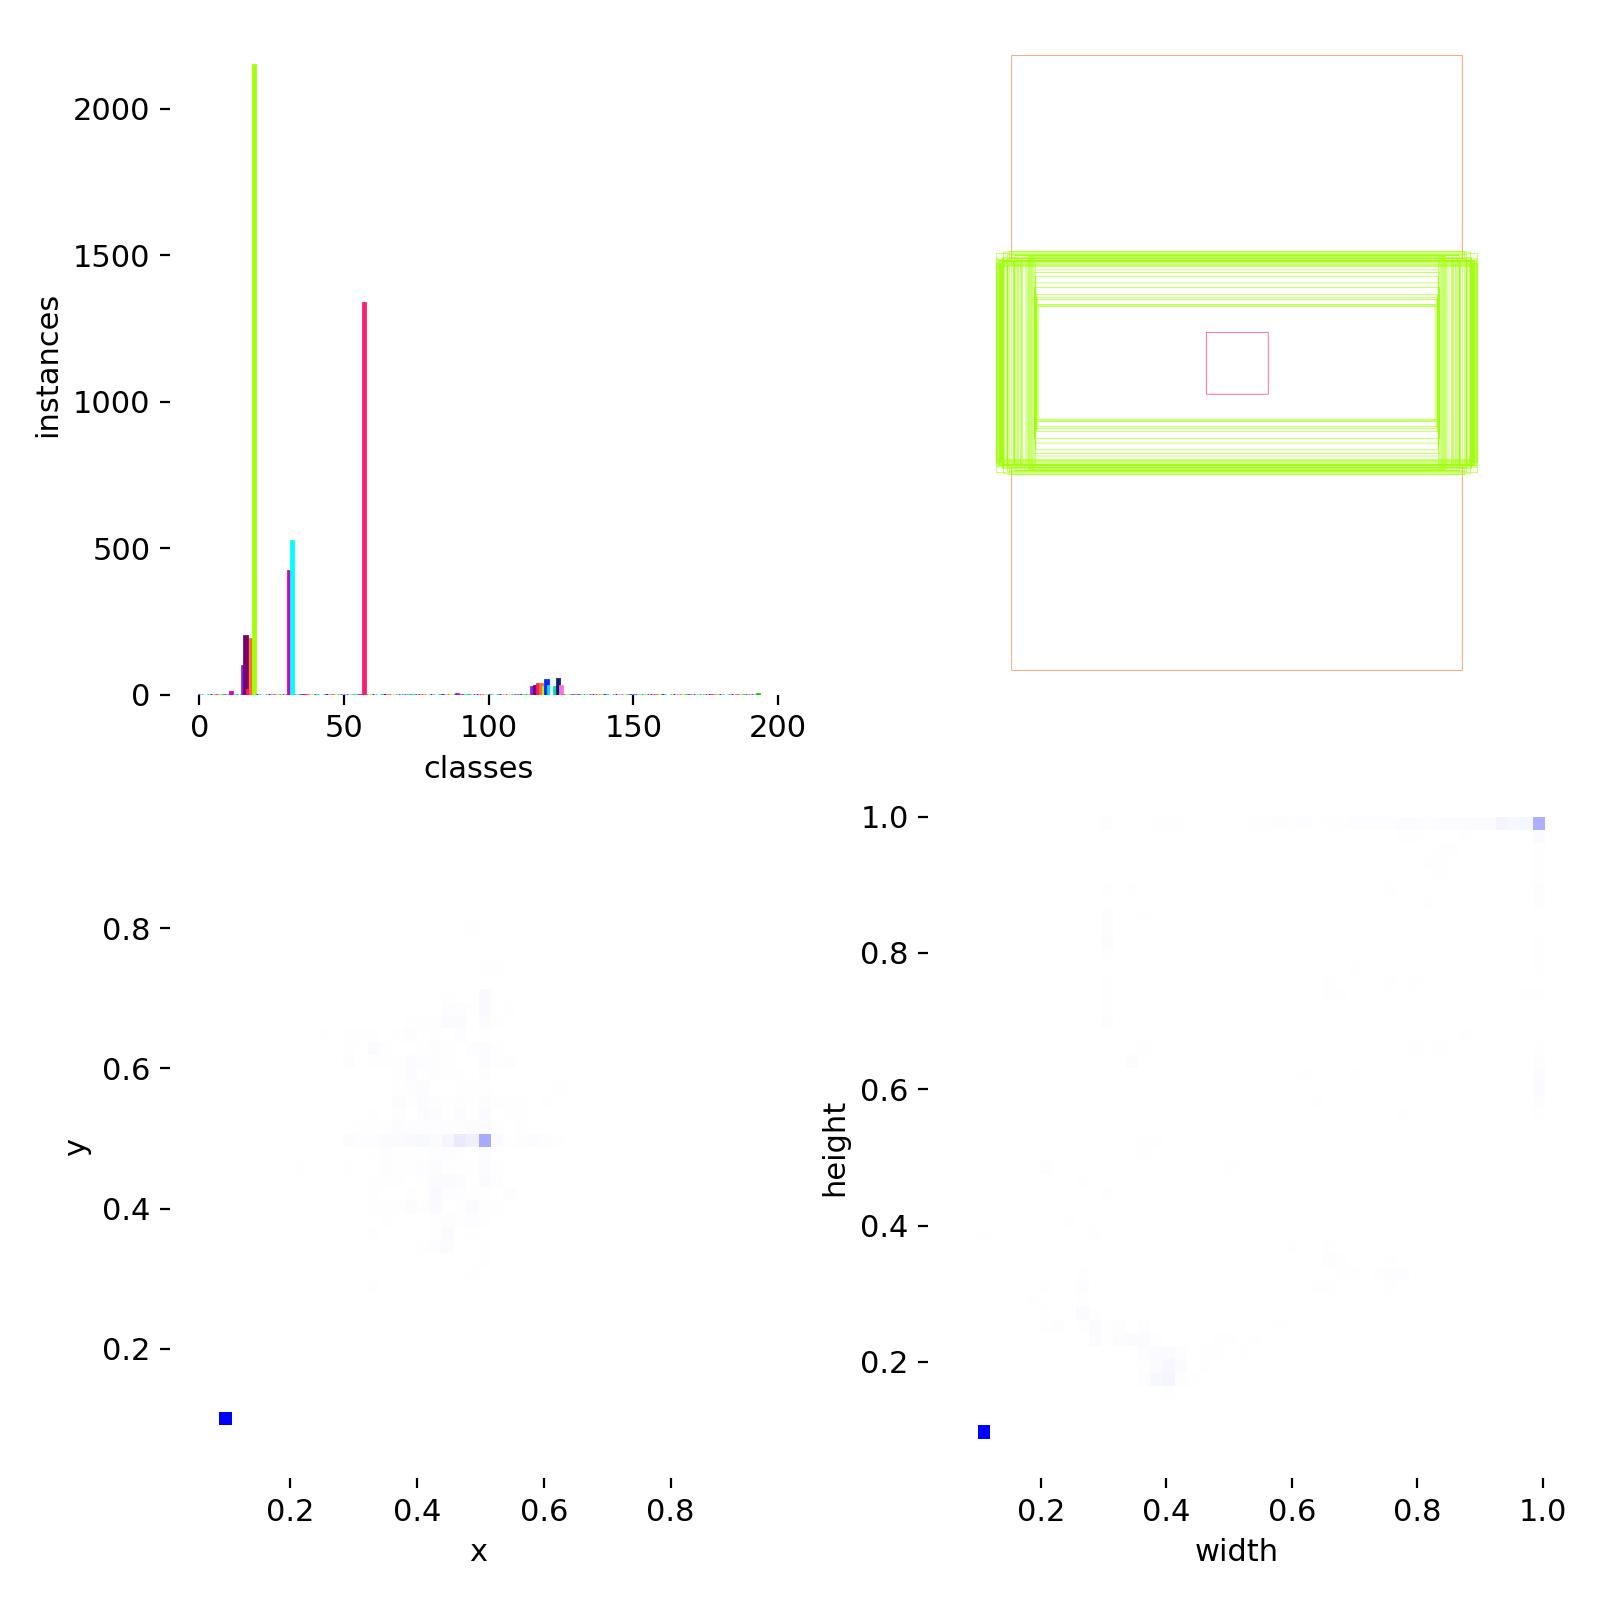
\includegraphics[width=0.62\textwidth]{task2_poi_xlarge/labels.jpg}
    \caption{Distribuzione delle istanze per classe (in alto a sinistra), distribuzione spaziale dei centri delle bounding box (in basso a sinistra) e distribuzione delle dimensioni (larghezza vs. altezza, in basso a destra). Si nota la forte disomogeneità tra le classi e la predominanza di bounding box di grandi dimensioni, tipiche dei POI architettonici.}
    \label{fig:labels_dist}
\end{figure}

\FloatBarrier

\subsection{Fase 2: Training}

L'addestramento è stato eseguito su un cluster HPC del Dipartimento di Matematica e Informatica (DMI) dell'Università di Catania, utilizzando GPU NVIDIA L40S tramite il sistema di job scheduling SLURM e il container runtime Apptainer.

Lo script \texttt{task2\_train\_yolo.py} sfrutta l'API della libreria \texttt{ultralytics} per configurare e lanciare l'addestramento caricando i pesi pre-addestrati sul dataset COCO.

La configurazione del job SLURM è stata definita nello script \texttt{run\_task2\_yolo.sh}, con le seguenti risorse allocate:
\begin{itemize}
    \item 1 GPU NVIDIA L40S (22 GB VRAM allocati tramite \texttt{gres=shard})
    \item 32 GB di RAM di sistema
    \item Timeout massimo di 12 ore
\end{itemize}

\section{Esperimenti e Risultati}

Sono stati condotti due esperimenti principali variando la capacità dell'architettura detector, al fine di analizzare in modo rigoroso il trade-off tra efficienza computazionale ed accuratezza di localizzazione.

\subsection{Setup Sperimentale}

Per valutare la scalabilità delle prestazioni, abbiamo configurato due run sperimentali sulla base dei modelli \textbf{YOLOv8n} (\emph{Nano}, $\sim$3.3M parametri) e \textbf{YOLOv8x} (\emph{X-Large}, $\sim$68.3M parametri). Entrambe le reti sono state inizializzate con pesi pre-addestrati sul benchmark COCO e ri-addestrate end-to-end sul dataset EGO-CH. La Tabella~\ref{tab:setup} sintetizza la configurazione e gli iperparametri adottati.

\begin{table}[htbp]
\centering
\caption{Configurazione degli esperimenti condotti per il Task 2.}
\label{tab:setup}
\begin{tabular}{lcc}
\toprule
\textbf{Parametro} & \textbf{Run 1 (Nano)} & \textbf{Run 2 (X-Large)} \\
\midrule
Architettura        & YOLOv8n              & YOLOv8x \\
Pesi iniziali       & \texttt{yolov8n.pt} (COCO) & \texttt{yolov8x.pt} (COCO) \\
Parametri           & $\sim$3.3 M          & $\sim$68.3 M \\
Epoche massime      & 100                  & 300 \\
Batch size          & 32                   & 16 \\
Risoluzione input   & $640 \times 640$     & $640 \times 640$ \\
Optimizer           & Auto (SGD)           & Auto (SGD) \\
Learning rate ($\text{lr}_0$) & 0.01       & 0.01 \\
Data augmentation   & Mosaic, RandAugment, Erasing & Mosaic, RandAugment, Erasing \\
Early stopping      & Patience = 100       & Patience = 100 \\
\bottomrule
\end{tabular}
\end{table}

\FloatBarrier

\subsection{Risultati Quantitativi}

La valutazione quantitativa sui dati di test del Monastero dei Benedettini conferma la drastica superiorità dell'approccio anchor-free basato su YOLOv8 rispetto alla baseline del paper originale. La Tabella~\ref{tab:results_main} riporta le metriche principali, mentre la Tabella~\ref{tab:improvement} riassume i miglioramenti percentuali relativi ottenuti.

\begin{table}[htbp]
\centering
\caption{Confronto delle performance di Object Detection sul Monastero dei Benedettini (la metrica mAP@50 consente il confronto diretto con la baseline YOLOv3). Vengono riportate anche le metriche COCO-style mAP@[50:95].}
\label{tab:results_main}
\begin{tabular}{lccc}
\toprule
\textbf{Metrica} & \textbf{Baseline YOLOv3 \cite{egoref}} & \textbf{YOLOv8n (Nano)} & \textbf{YOLOv8x (X-Large)} \\
\midrule
\textbf{mAP@50}         & 15.45\%   & 19.92\%   & \textbf{29.70\%} \\
mAP@[50:95]     & ---       & 14.82\%   & \textbf{24.30\%} \\
Precision       & ---       & 0.489     & \textbf{0.685}   \\
Recall          & ---       & 0.218     & \textbf{0.298}   \\
\midrule
Parametri       & $\sim$61 M & $\sim$3.3 M & $\sim$68.3 M \\
Epoche effettive & ---      & 100/100   & 269/300 (early stop) \\
Tempo di training & ---     & $\sim$1.6 ore & $\sim$7.2 ore \\
\bottomrule
\end{tabular}
\end{table}

\begin{table}[htbp]
\centering
\caption{Incrementi relativi della mAP@50 rispetto alla baseline YOLOv3 del paper originale ($15.45\%$).}
\label{tab:improvement}
\begin{tabular}{lcc}
\toprule
\textbf{Modello} & \textbf{mAP@50} & \textbf{$\Delta$ relativo vs. Baseline} \\
\midrule
Baseline YOLOv3 (Paper) & 15.45\% & --- \\
YOLOv8n (Nano)          & 19.92\% & \textbf{+28.9\%} \\
YOLOv8x (X-Large)       & 29.70\% & \textbf{+92.2\%} \\
\bottomrule
\end{tabular}
\end{table}

\FloatBarrier

\subsection{Curve di Addestramento}

L'analisi dell'andamento delle funzioni di perdita (\emph{box loss}, \emph{classification loss}, \emph{distribution focal loss}) e delle metriche di validazione fornisce utili indicazioni sulla dinamica di convergenza dei due modelli. La Figura~\ref{fig:results_nano} mostra l'evoluzione per il modello Nano, mentre la Figura~\ref{fig:results_xlarge} illustra l'addestramento della rete X-Large.

\begin{figure}[htbp]
    \centering
    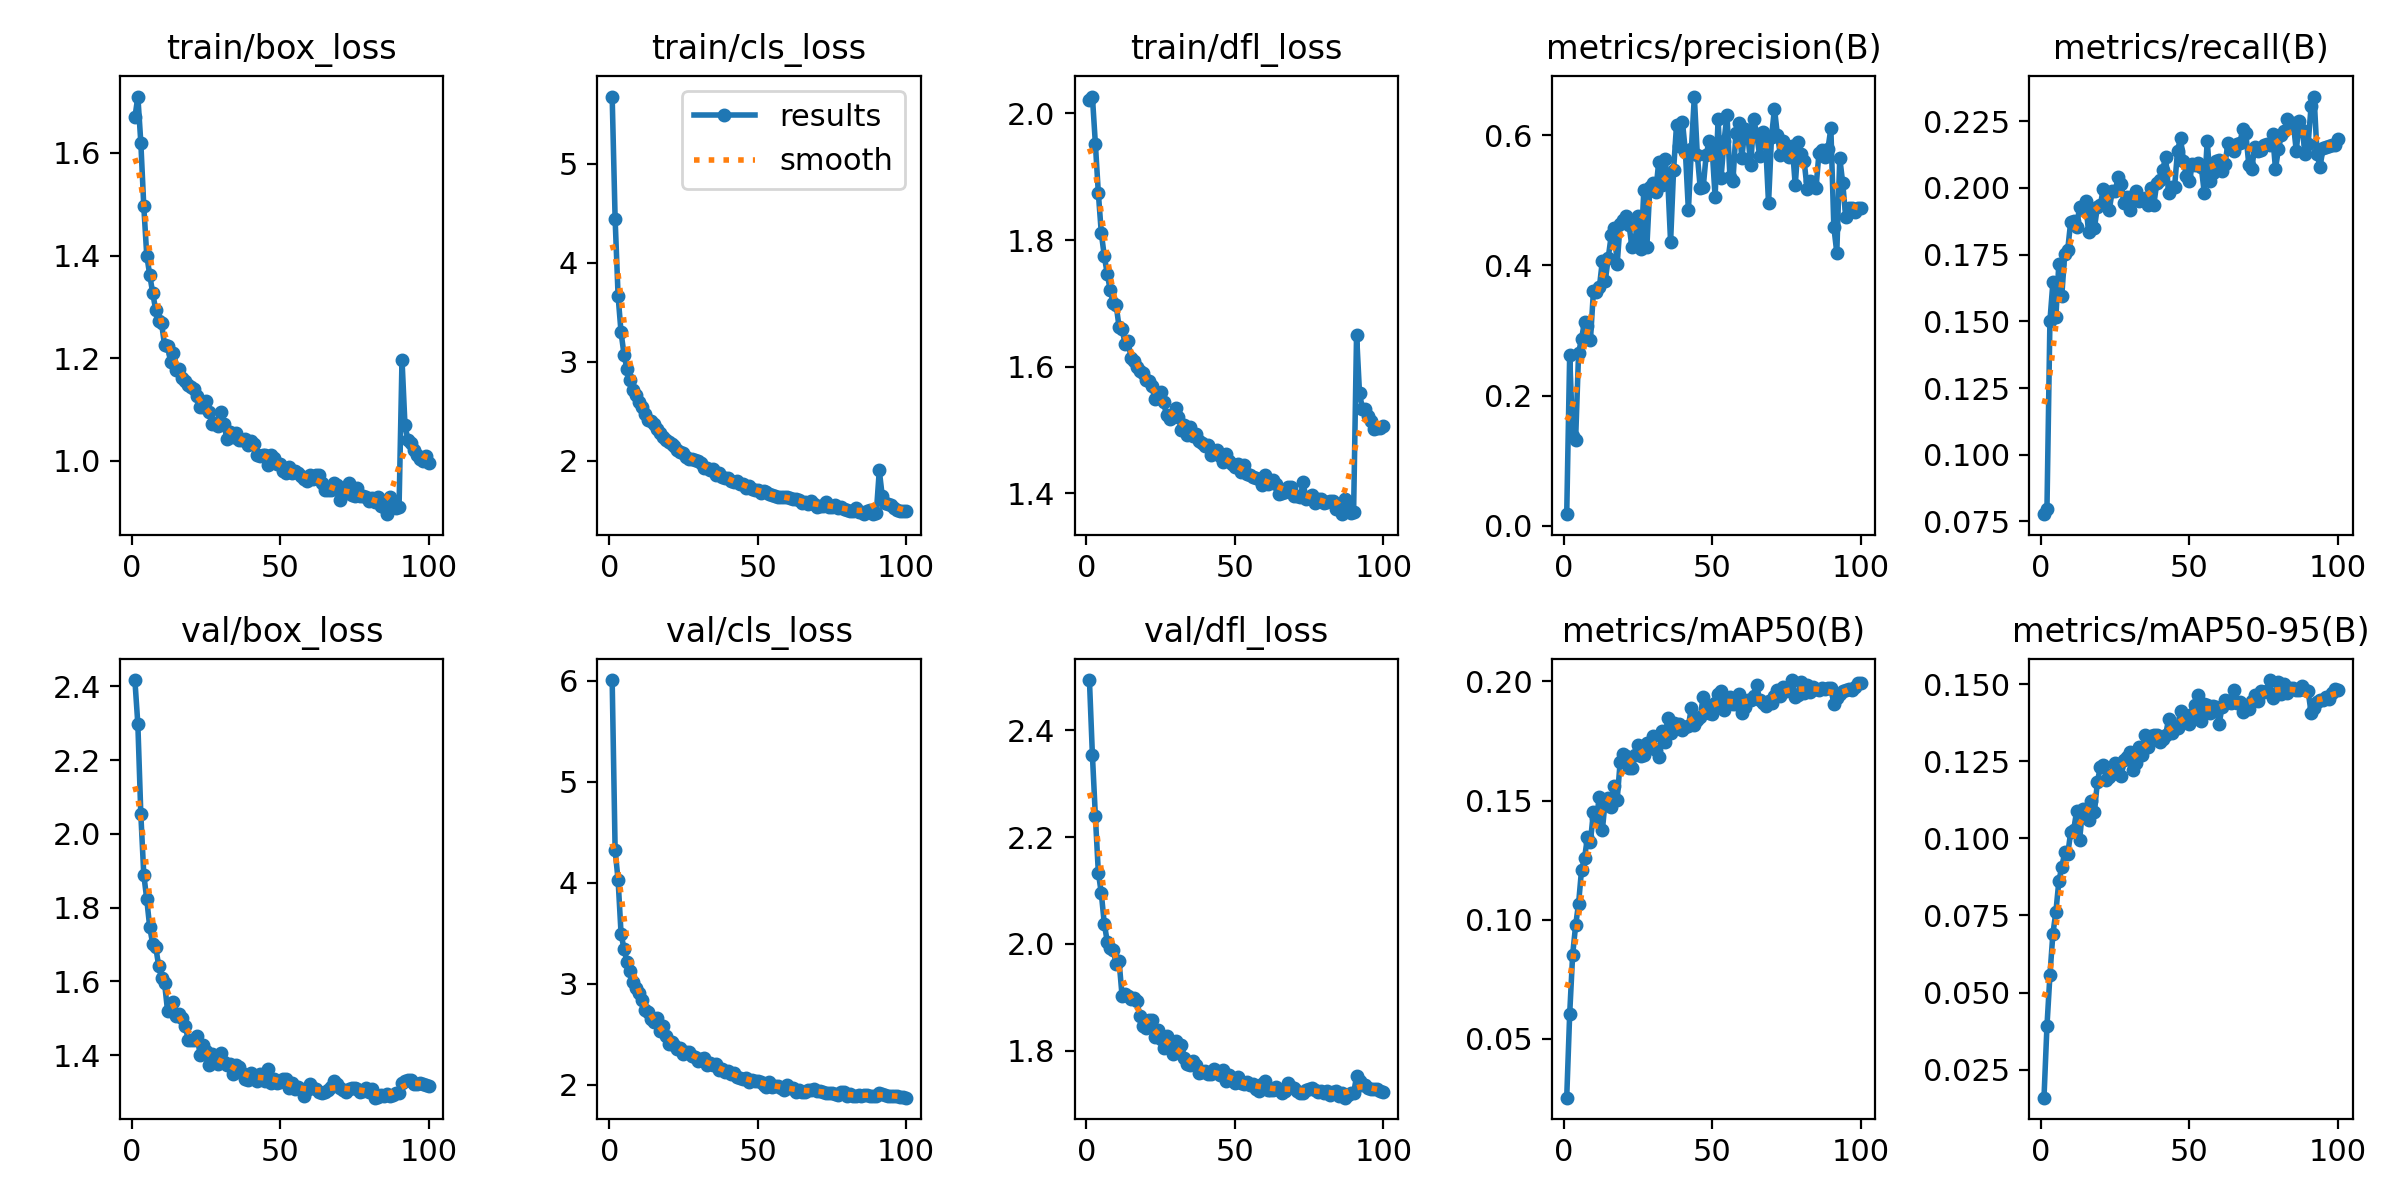
\includegraphics[width=0.72\textwidth]{task2_poi/results.png}
    \caption{Curve di addestramento del modello YOLOv8n (Nano, 100 epoche). Le loss di training (box, cls, dfl) mostrano una convergenza regolare, mentre le metriche di validazione (mAP@50 e mAP@50-95) evidenziano un aumento costante fino all'ultima epoca, suggerendo che il modello avrebbe potuto beneficiare di un addestramento più lungo.}
    \label{fig:results_nano}
\end{figure}

\begin{figure}[htbp]
    \centering
    
\includegraphics[width=0.72\textwidth]{task2_poi_xlarge/results.png}
    \caption{Curve di addestramento del modello YOLOv8x (X-Large, 269 epoche su 300 massime). Si osserva una convergenza più lenta ma più ricca: le loss di validazione raggiungono un plateau intorno all'epoca 100, mentre le metriche mAP continuano a crescere fino all'epoca $\sim$170, dopo la quale il meccanismo di early stopping (patience = 100) arresta l'addestramento all'epoca 269.}
    \label{fig:results_xlarge}
\end{figure}

\FloatBarrier

\subsection{Analisi Qualitativa}

Per verificare l'efficacia pratica della localizzazione, la Figura~\ref{fig:qualitative} propone un confronto affiancato tra le annotazioni manuali di \emph{ground truth} e le predizioni generate dal modello YOLOv8x su un batch di immagini di validazione. Si nota la capacità della rete di isolare POI complessi anche in presenza di forte prospettiva ed ambienti poco illuminati.

\begin{figure}[htbp]
    \centering
    \begin{subfigure}[b]{0.48\textwidth}
        \centering
        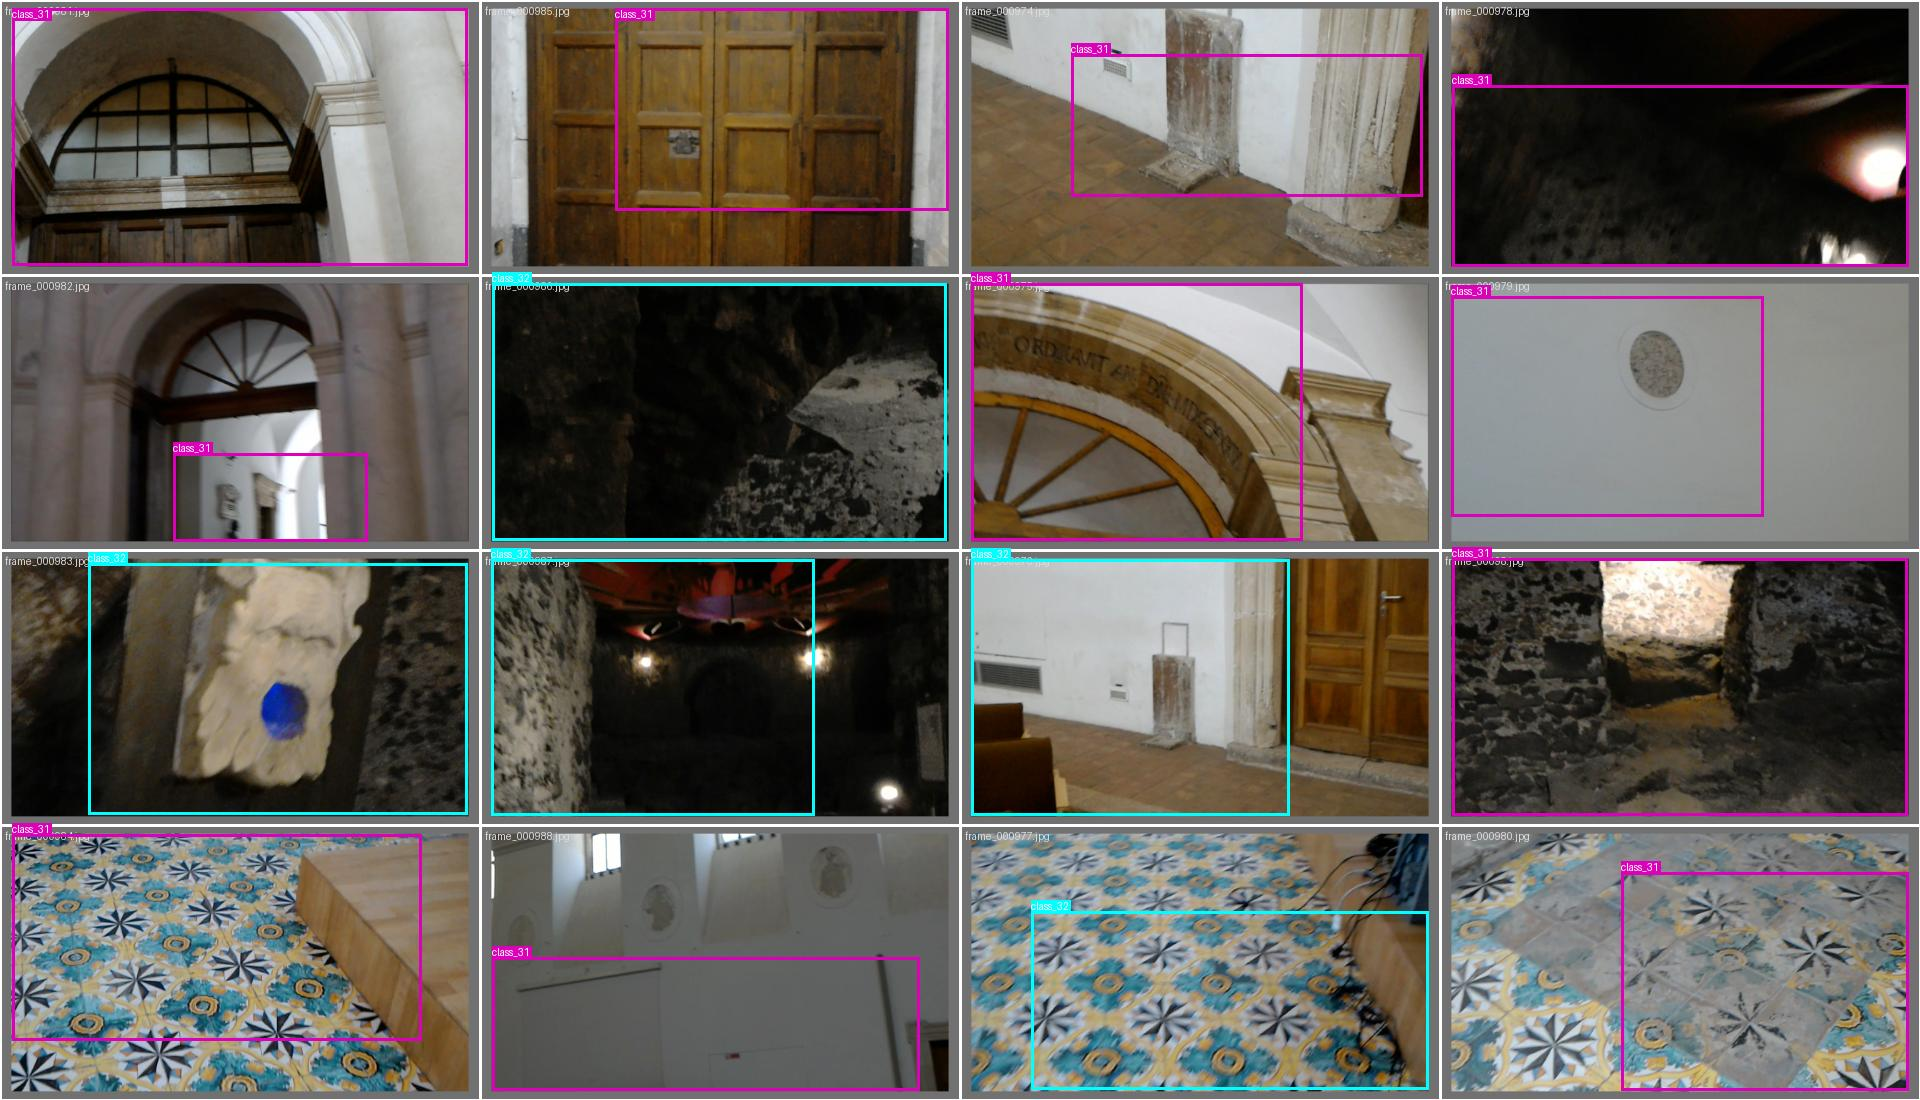
\includegraphics[width=\textwidth]{task2_poi_xlarge/val_batch0_labels.jpg}
        \caption{Ground truth: BB manuali.}
    \end{subfigure}
    \hfill
    \begin{subfigure}[b]{0.48\textwidth}
        \centering
        
\includegraphics[width=\textwidth]{task2_poi_xlarge/val_batch0_pred.jpg}
        \caption{Predizioni YOLOv8x.}
    \end{subfigure}
    \caption{Confronto qualitativo tra ground truth (a) e predizioni YOLOv8x (b) su un batch di validazione. Le bounding box colorate indicano le classi dei POI. Si noti la varietà delle scene: archi, porte, pavimenti maiolicati, ambienti bui --- tutti elementi tipici della sfida egocentrica in contesti culturali.}
    \label{fig:qualitative}
\end{figure}

\FloatBarrier

\subsection{Matrice di Confusione}

Per studiare il comportamento per-classe del detector e identificare eventuali sbilanciamenti, la Figura~\ref{fig:confusion} illustra la matrice di confusione normalizzata per il modello YOLOv8x. Si osserva la pronunciata sparsità della diagonale, dovuta alla prevalenza di classi dominanti a discapito di quelle rare.

\begin{figure}[htbp]
    \centering
    
\includegraphics[width=0.65\textwidth]{task2_poi_xlarge/confusion_matrix_normalized.png}
    \caption{Matrice di confusione normalizzata del modello YOLOv8x. La forte sparsità della matrice riflette il numero elevatissimo di classi ($>$60) e la distribuzione long-tail del dataset: solo poche classi ben rappresentate (class\_15, class\_16, class\_57) mostrano attivazioni significative sulla diagonale, mentre la maggior parte delle classi rare non viene mai predetta.}
    \label{fig:confusion}
\end{figure}

\FloatBarrier

\section{Discussione}

\subsection{Confronto con la Baseline del Paper}

Il confronto con la baseline del paper originale rivela due risultati significativi:

\paragraph{YOLOv8n supera la baseline con 20$\times$ meno parametri.}
Il modello Nano ha ottenuto un mAP@50 di \textbf{19.92\%}, superiore del \textbf{+28.9\%} rispetto al 15.45\% di YOLOv3, pur disponendo di soli 3.3M di parametri contro i 61M del baseline. Questo risultato dimostra che le innovazioni architetturali di YOLOv8 (come l'approccio anchor-free e la struttura modernizzata) non solo compensano la riduzione drastica di capacità, ma portano a un netto miglioramento delle performance.

Il modello Nano risulta particolarmente adatto a scenari di deployment in tempo reale su dispositivi edge (es. visori HoloLens, smartphone), dove la potenza computazionale e il consumo energetico sono vincoli stringenti.

\paragraph{YOLOv8x raddoppia le performance della baseline.}
Il modello X-Large ha raggiunto un mAP@50 di \textbf{29.70\%}, segnando un incremento relativo del \textbf{+92.2\%} rispetto alla baseline. L'analisi dettagliata evidenzia:

\begin{itemize}
    \item \textbf{Risoluzione dell'ambiguità visiva}: l'architettura anchor-free, combinata con il backbone CSPDarknet a piena capacità, ha permesso al modello di discriminare efficacemente tra POI visivamente simili.
    
    \item \textbf{Performance per classe non uniformi}: la rete X-Large ha raggiunto precisioni quasi perfette su classi ben rappresentate (es. Class\_16: mAP 95.2\%, Class\_15: mAP 82.4\%), mentre le classi con poche istanze o alta ambiguità visiva restano problematiche. Questa distribuzione long-tail è un limite intrinseco del dataset.
    
    \item \textbf{Early stopping funzionale}: l'addestramento si è arrestato automaticamente all'epoca 269 (su un massimo di 300), indicando che il modello ha raggiunto la convergenza intorno all'epoca 169 senza overfitting distruttivo.
    
    \item \textbf{Robustezza al motion blur}: la maggiore capacità di estrazione delle feature del backbone X-Large ha permesso di gestire il motion blur tipico dei video egocentrici in modo significativamente più robusto rispetto a YOLOv3.
\end{itemize}

\subsection{Nota sulla Comparabilità delle Metriche}

È importante sottolineare che il paper originale riporta la metrica \textbf{mAP@50} (IoU threshold = 0.5), che è la metrica standard per YOLOv3. I nostri risultati vengono riportati sia in formato mAP@50 (per il confronto diretto) sia nel formato COCO-style \textbf{mAP@[50:95]} (media su 10 soglie IoU da 0.5 a 0.95 con passo 0.05), che è lo standard moderno e produce valori sistematicamente inferiori in quanto più stringente. Il confronto diretto sulla metrica mAP@50 è il più corretto e mostra il miglioramento nella sua interezza.

\subsection{Trade-off Efficienza--Accuratezza}

Il confronto tra i due modelli mette in luce un chiaro trade-off:

\begin{itemize}
    \item Se l'obiettivo è l'\textbf{accuratezza massima} per una valutazione accademica o per un sistema di analisi offline, \textbf{YOLOv8x} stabilisce il nuovo stato dell'arte con un margine netto.
    \item Se l'obiettivo prevede il \textbf{deployment su dispositivi indossabili} con risorse limitate, \textbf{YOLOv8n} offre un compromesso eccezionale, superando la precisione del baseline originale con una frazione dei parametri e un'inferenza in tempo reale.
\end{itemize}

% ================================================================
% CAPITOLO 5 — TASK 3: OBJECT RETRIEVAL
% ================================================================
\chapter{Task 3 --- Object Retrieval}

\section{Definizione del Problema}

Il Task 3, denominato \emph{Object Retrieval}, consiste nel recuperare l'immagine di riferimento di uno specifico Punto di Interesse (POI) da un database (Gallery), a partire da un'immagine di \emph{query} ritagliata che contiene il medesimo oggetto.

Nel contesto della \emph{Egocentric Vision} applicata ai beni culturali, questo task riveste una notevole rilevanza pratica: permette infatti l'identificazione automatica e il recupero di schede informative relative a un'opera d'arte quando la fase di \emph{object detection} può essere bypassata --- ad esempio quando il visitatore inquadra spontaneamente l'opera ponendola al centro del campo visivo del visore indossabile o dello smartphone. Inoltre, come evidenziato nei capitoli precedenti, il rilevamento spaziale preciso dei POI (Task 2) rappresenta una sfida estremamente complessa; l'Object Retrieval offre pertanto una formulazione alternativa e complementare focalizzata direttamente sul matching visivo.

\subsection{Formulazione One-Shot Retrieval}

In conformità con il protocollo sperimentale definito nel benchmark EGO-CH~\cite{egoref}, abbiamo concentrato le nostre analisi sulla formulazione più critica e sfidante: il \textbf{One-Shot Retrieval}.
In questa variante:
\begin{itemize}
    \item \textbf{Gallery (Database di Riferimento)}: contiene esclusivamente le immagini di riferimento pulite e ufficiali associati a ciascun POI (una sola immagine per ogni classe). Tali immagini provengono dalla cartella \texttt{Training/} di ciascun sito culturale.
    \item \textbf{Query (Set di Test)}: è costituito dall'insieme di tutte le patch visive ritagliate dai bounding box annotati nei video di visita egocentrica (contenute nella cartella \texttt{Test/}). Nello specifico, si tratta di \textbf{23.727 patch} per Palazzo Bellomo e \textbf{44.978 patch} per il Monastero dei Benedettini.
\end{itemize}

\subsection{Le Sfide del Domain Shift}

La formulazione One-Shot introduce due insidie fondamentali:
\begin{enumerate}
    \item \textbf{Estrema scarsità di campioni etichettati}: il modello ha a disposizione una sola immagine di esempio per ciascuna classe nella Gallery per apprendere o confrontare la rappresentazione dell'oggetto.
    \item \textbf{Marcato Domain Shift (Disallineamento di Dominio)}: esiste una drastica differenza qualitativa e geometrica tra le immagini della Gallery (fotografie da catalogo professionale, ben illuminate, perfettamente a fuoco e frontali) e le immagini Query (ritagli di fotogrammi egocentrici caratterizzati da sfocature da movimento, occlusioni parziali, prospettive angolate, riflessi e variazioni estreme di luce ambientale).
\end{enumerate}

\section{La Baseline del Paper Originale}

\subsection{Architettura e Metodologia}

Nella baseline proposta dagli autori di EGO-CH~\cite{egoref}, l'estrazione delle caratteristiche visive dalle patch viene affidata a una rete \textbf{VGG19} pre-addestrata in modo supervisionato su ImageNet. Le feature vengono prelevate dal penultimo strato fully-connected (\texttt{FC7}), ottenendo vettori di rappresentazione a 4096 dimensioni.

Il matching tra la query e le immagini del database viene eseguito mediante l'algoritmo \textbf{K-Nearest Neighbors (K-NN)} con $K=1$, misurando la vicinanza nello spazio euclideo delle feature estratte.

\subsection{Risultati del Paper (Tabella 5)}

La Tabella~\ref{tab:baseline_retrieval_paper} riassume i risultati ottenuti dalla baseline VGG19 nella variante One-Shot per i due siti culturali, così come riportati nella Tabella~5 del paper originale.

\begin{table}[htbp]
\centering
\caption{Risultati della baseline VGG19 (FC7 + 1-NN) dal paper EGO-CH~\cite{egoref} per il One-Shot Retrieval (Tabella 5).}
\label{tab:baseline_retrieval_paper}
\begin{tabular}{lccc}
\toprule
\textbf{Sito Culturale} & \textbf{Precision} & \textbf{Recall} & \textbf{F1 Score} \\
\midrule
Monastero dei Benedettini (35 POI) & 0.290 & 0.070 & 0.080 \\
Palazzo Bellomo (191 POI)          & 0.004 & 0.007 & 0.001 \\
\bottomrule
\end{tabular}
\end{table}

\subsection{Criticità della Baseline}

I risultati evidenziano come la baseline basata su VGG19 fallisca nel gestire l'impatto del One-Shot Retrieval:
\begin{itemize}
    \item Nel \textbf{Monastero dei Benedettini}, nonostante il contenuto numero di classi (35 POI), la F1 Score si arresta a un modestissimo $0.080$, penalizzata da una Recall bassissima ($0.070$).
    \item A \textbf{Palazzo Bellomo}, con 191 POI visivamente simili, la baseline crolla completamente a una F1 Score pari a $0.001$, valore pressoché indistinguibile dalla scelta casuale ($1/191 \approx 0.005$). Ciò dimostra la totale incapacità delle feature \texttt{FC7} di VGG19 di superare il \emph{domain shift} e discriminare tra istanze di opere d'arte in presenza di un solo campione di riferimento.
\end{itemize}

\section{La Nostra Proposta: DINOv2 e Matching Latente}

\subsection{Motivazione dell'Estrattore Vision Transformer}

Per superare i limiti strutturali della baseline convoluzionale, abbiamo progettato una pipeline basata sul foundation model \textbf{DINOv2} (\texttt{dinov2\_vits14})~\cite{dinov2}. 

A differenza delle CNN tradizionali addestrate per classificazione supervisionata su ImageNet (che tendono a concentrarsi su scorciatoie tessiturali o sull'oggetto dominante della classe), DINOv2 viene addestrato con tecniche di \emph{Self-Supervised Learning} (SSL) che incoraggiano la rete ad apprendere concetti semantici e geometrici profondi. Le motivazioni chiave per l'adozione di DINOv2 nel retrieval One-Shot sono:

\begin{enumerate}
    \item \textbf{Invarianza alle Trasformazioni visive}: gli obiettivi di apprendimento auto-supervisionato di DINOv2 garantiscono che l'embedding di un oggetto rimanga stabile nello spazio latente anche in presenza di variazioni di scala, illuminazione, sfocatura o punto di vista.
    \item \textbf{Rappresentazione Densa e Compatta}: la variante \texttt{dinov2\_vits14} (Vision Transformer Small con patch da $14 \times 14$ pixel) genera per ogni patch un vettore descrittore denso di dimensione \textbf{384}, drasticamente più compatto rispetto ai 4096 valori di VGG19 FC7.
\end{enumerate}

\subsection{Metriche di Matching: Cosine Similarity}

In luogo di un classificatore supervisionato a valle o di una distanza euclidea semplice, il matching tra la query egocentrica e l'insieme delle immagini della Gallery viene calcolato direttamente nello spazio latente di DINOv2 tramite la \textbf{Cosine Similarity}:

\begin{equation}
\text{sim}(\mathbf{q}, \mathbf{g}_i) = \frac{\mathbf{q} \cdot \mathbf{g}_i}{\|\mathbf{q}\|_2 \|\mathbf{g}_i\|_2}
\end{equation}

dove $\mathbf{q} \in \mathbb{R}^{384}$ rappresenta l'embedding della patch Query ed $\mathbf{g}_i \in \mathbb{R}^{384}$ è l'embedding dell'i-esimo elemento della Gallery. Per ciascuna query, l'etichetta predetta corrisponde al POI dell'immagine in Gallery che massimizza la similitudine coseno:

\begin{equation}
\hat{y} = \arg\max_{i} \, \text{sim}(\mathbf{q}, \mathbf{g}_i)
\end{equation}

Questo approccio sfrutta l'orientamento dei vettori nello spazio delle caratteristiche di DINOv2, risultando insensibile alle variazioni di norma indotte da differenze di contrasto o luminosità tra le immagini.

\section{Pipeline Implementativa}

La pipeline di Object Retrieval è stata strutturata in script Python modulari, progettati per garantire l'esecuzione efficiente su architetture HPC (cluster GCluster dell'Università di Catania):

\begin{enumerate}
    \item \textbf{\texttt{task3\_extract\_patch\_features.py}}:
    \begin{itemize}
        \item Riceve in ingresso il percorso delle patch ritagliate (\texttt{patches\_dir}) e il file di output \texttt{.pt}.
        \item Ridimensiona le immagini alla risoluzione di $224 \times 224$ e applica le trasformazioni di normalizzazione standard di ImageNet ($\mu = [0.485, 0.456, 0.406]$, $\sigma = [0.229, 0.224, 0.225]$).
        \item Carica il modello \texttt{dinov2\_vits14} in modalità offline e disabilita il calcolo dei gradienti (\texttt{torch.no\_grad()}).
        \item Estrae i vettori latenti a 384 dimensioni per tutte le immagini della Gallery e delle Query, salvando su disco un dizionario PyTorch contenente l'associazione \texttt{percorso\_relativo $\rightarrow$ tensore}.
    \end{itemize}

    \item \textbf{\texttt{task3\_evaluate\_retrieval.py}}:
    \begin{itemize}
        \item Carica i file delle feature estratte (\texttt{gallery\_features.pt} e \texttt{query\_features.pt}) unitamente alle etichette ufficiali (\texttt{labels.txt}).
        \item Associa a ciascun frame di query la relativa etichetta di \emph{ground truth} leggendo le annotazioni contenute nella cartella \texttt{Test/labels}.
        \item Calcola in maniera massiva e vettorizzata la matrice di Cosine Similarity di forma $N_{\text{queries}} \times N_{\text{gallery}}$ sfruttando le funzioni ottimizzate di \texttt{scikit-learn}.
        \item Valuta le metriche di accuratezza e le metriche pesate (\emph{weighted}) di Precision, Recall e F1 Score per un confronto diretto con la letteratura.
    \end{itemize}

    \item \textbf{Script di Orchestrazione SLURM (\texttt{run\_task3.sh} / \texttt{task3.sh})}:
    \begin{itemize}
        \item Automatizzano l'esecuzione della pipeline su nodi computazionali dotati di GPU NVIDIA L40S all'interno di ambienti containerizzati Apptainer.
    \end{itemize}
\end{enumerate}

\section{Esperimenti e Risultati}

La Tabella~\ref{tab:task3_results_comparison} riporta il confronto sistematico tra la baseline VGG19 pubblicata nel paper EGO-CH e la nostra soluzione basata su DINOv2 per entrambi i siti culturali nella formulazione One-Shot Retrieval.

\begin{table}[htbp]
\centering
\caption{Confronto delle performance di One-Shot Retrieval tra la baseline VGG19 del paper EGO-CH~\cite{egoref} e la nostra architettura DINOv2 (\texttt{dinov2\_vits14} + Cosine Similarity).}
\label{tab:task3_results_comparison}
\resizebox{\textwidth}{!}{%
\begin{tabular}{lcccc}
\toprule
\textbf{Sito / Modello} & \textbf{Precision} & \textbf{Recall} & \textbf{F1 Score} & \textbf{Accuracy} \\
\midrule
\multicolumn{5}{l}{\textbf{Monastero dei Benedettini (35 POI)}} \\
Baseline VGG19 (Paper) & 0.2900 & 0.0700 & 0.0800 & --- \\
\textbf{Nostro Modello (DINOv2)} & \textbf{0.5353} & \textbf{0.3369} & \textbf{0.3752} & \textbf{0.3369} \\
\textit{Incremento Relativo} & \textit{+84.6\%} & \textit{+381.3\%} & \textit{\textbf{+369.0\%}} & --- \\
\midrule
\multicolumn{5}{l}{\textbf{Palazzo Bellomo (191 POI)}} \\
Baseline VGG19 (Paper) & 0.0040 & 0.0070 & 0.0010 & --- \\
\textbf{Nostro Modello (DINOv2)} & \textbf{0.2194} & \textbf{0.1643} & \textbf{0.1512} & \textbf{0.1643} \\
\textit{Incremento Relativo} & \textit{+54.8$\times$} & \textit{+23.5$\times$} & \textit{\textbf{+151.2$\times$}} & --- \\
\bottomrule
\end{tabular}%
}
\end{table}

\section{Discussione e Analisi Comparativa}

L'analisi comparativa dei risultati sperimentali permette di trarre importanti conclusioni di carattere metodologico e architetturale.

\subsection{Risoluzione del Domain Shift mediante SSL}

Il risultato di maggior rilievo è rappresentato dall'incredibile incremento delle prestazioni ottenuto su entrambi i dataset:
\begin{itemize}
    \item Nel \textbf{Monastero dei Benedettini}, DINOv2 fa registrare un aumento della F1 Score da $0.0800$ a $0.3752$ (un fattore di incremento pari a quasi \textbf{$5\times$}), raddoppiando contestualmente la Precision ($0.5353$ vs $0.2900$).
    \item A \textbf{Palazzo Bellomo}, la baseline VGG19 soffriva un crollo catastrofico ($F1 = 0.0010$), rendendo il task sostanzialmente inaffrontabile. DINOv2 eleva la F1 Score al \textbf{$15.12\%$} ($0.1512$), con un incremento superiore a \textbf{$150$ volte}.
\end{itemize}

Questi miglioramenti confermano l'ipotesi che la rappresentazione latente di DINOv2 sia intrinsecamente immune alle discrepanze di dominio. Le caratteristiche visive estratte da VGG19, legate a filtri convoluzionali rigidi addestrati su classi ImageNet ad alto livello, falliscono nel momento in cui devono confrontare una fotografia di catalogo ideale con un ritaglio egocentrico sfocato e angolato. Al contrario, l'architettura Vision Transformer di DINOv2 apprende mappe di attenzione locali e globali che isolano le strutture geometriche invarianti dell'opera d'arte.

\subsection{Efficienza Computazionale e Spaziale}

Oltre alla drastica superiorità in accuratezza, l'approccio proposto si dimostra notevolmente più efficiente dal punto di vista infrastrutturale:
\begin{itemize}
    \item \textbf{Dimensione dei Vettori}: il passaggio da vettori a 4096 dimensioni (VGG19 \texttt{FC7}) a vettori da 384 dimensioni (DINOv2 \texttt{ViT-S/14}) comporta una \textbf{riduzione dell'occupazione di memoria superiore al 90\%} sia su disco che in RAM VRAM.
    \item \textbf{Velocità di Matching}: la riduzione della dimensionalità consente di calcolare le matrici di Cosine Similarity tra decine di migliaia di vettori di query ($>44.000$ patch nel Monastero) e il database della Gallery in pochi millisecondi su architetture hardware standard, rendendo il sistema adatto all'impiego in tempo reale su dispositivi wearable.
\end{itemize}

\subsection{Impatto della Scalabilità e della Complessità dei Siti}

Infine, i risultati evidenziano la netta differenza di difficoltà tra i due contesti culturali. Palazzo Bellomo presenta un numero di POI oltre 5 volte superiore rispetto al Monastero (191 vs 35 classi), molti dei quali visivamente simili (es. dipinti sacri dello stesso periodo storico o con soggetti analoghi). Nonostante la complessità intrinseca di Palazzo Bellomo mantenga i punteggi assoluti inferiori rispetto al Monastero, l'adozione di DINOv2 dimostra che una rappresentazione latente auto-supervisionata consente di estrarre un segnale discriminativo affidabile anche in scenari ad elevata cardinalità di classe.

% ================================================================
% CAPITOLO 6 — CONCLUSIONI
% ================================================================
\chapter{Conclusioni}

La presente ricerca ha affrontato in maniera organica e approfondita i tre task fondamentali introdotti dal benchmark \textbf{EGO-CH} per la comprensione automatica del comportamento del visitatore in siti culturali mediante visione egocentrica.

Per ciascun task, l'adozione di metodologie di Deep Learning di ultima generazione ha consentito di superare in modo netto le baseline pubblicate nel paper originale di Ragusa et al. (2020):

\begin{enumerate}
    \item \textbf{Task 1 --- Room-based Localization}: la combinazione delle feature visive di DINOv2 con l'architettura di sequence modeling \textbf{Mamba} (State Space Model) ha permesso di modellare la continuità temporale della visita. L'introduzione della loss pesata, del label smoothing e dell'ottimizzazione dinamica del filtro mediano ha condotto al raggiungimento di un \textbf{FF1 di 0.8572} e di un \textbf{ASF1 di 0.6194} (modello V2), superando lo stato dell'arte sia a livello di singolo frame che di coerenza sequenziale.
    
    \item \textbf{Task 2 --- Point of Interest Recognition}: la sostituzione dell'architettura legacy YOLOv3 con il moderno detector anchor-free \textbf{YOLOv8} ha prodotto progressi straordinari. Il modello leggero \textbf{YOLOv8n} ha superato la baseline con un $20\times$ in meno di parametri ($19.92\%$ mAP@50), mentre il modello a piena capacità \textbf{YOLOv8x} ha quasi raddoppiato la precisione della baseline raggiungendo un \textbf{mAP@50 del 29.70\%} ($+92.2\%$ relativo).
    
    \item \textbf{Task 3 --- Object Retrieval}: la sostituzione dell'estrattore VGG19 con il foundation model \textbf{DINOv2} accoppiato alla similarità coseno nello spazio latente ha risolto in modo radicale il problema del \emph{Domain Shift} nel regime One-Shot. I risultati hanno registrato un incremento della F1 Score di quasi $5\times$ sul Monastero dei Benedettini ($0.3752$) e di oltre \textbf{$150\times$} su Palazzo Bellomo ($0.1512$), stabilendo un nuovo punto di riferimento per il retrieval One-Shot in contesti egocentrici.
\end{enumerate}

In conclusione, le evidenze sperimentali raccolte confermano che l'integrazione di foundation model basati su Vision Transformer (DINOv2), modelli temporali a spazio di stato (Mamba) e object detector anchor-free di ultima generazione (YOLOv8) permette di compiere un salto qualitativo decisivo nell'analisi di video egocentrici per i beni culturali, offrendo basi solide e ad alte prestazioni per lo sviluppo di guide intelligenti e sistemi d'assistenza di nuova generazione.

% ================================================================
% BIBLIOGRAFIA
% ================================================================
\begin{thebibliography}{9}

\bibitem{egoref}
F.~Ragusa, A.~Furnari, S.~Battiato, G.~Signorello, G.~M.~Farinella,
\textit{EGO-CH: Dataset and Fundamental Tasks for Visitors Behavioral Understanding using Egocentric Vision},
Pattern Recognition Letters, vol.~131, pp.~150--157, 2020.

\bibitem{yolov3}
J.~Redmon, A.~Farhadi,
\textit{YOLOv3: An Incremental Improvement},
arXiv preprint arXiv:1804.02767, 2018.

\bibitem{yolov8}
G.~Jocher, A.~Chaurasia, J.~Qiu,
\textit{Ultralytics YOLOv8},
\url{https://github.com/ultralytics/ultralytics}, 2023.

\bibitem{dinov2}
M.~Oquab et al.,
\textit{DINOv2: Learning Robust Visual Features without Supervision},
Transactions on Machine Learning Research, 2024.

\bibitem{mamba}
A.~Gu, T.~Dao,
\textit{Mamba: Linear-Time Sequence Modeling with Selective State Spaces},
arXiv preprint arXiv:2312.00752, 2023.

\end{thebibliography}

\end{document}

